\documentclass[11pt,a4paper]{article}

\usepackage[utf8]{inputenc}
\usepackage[T1]{fontenc}

\usepackage{amsfonts}
\usepackage{amsmath}
\usepackage{amssymb}
\usepackage{booktabs}
\usepackage{caption}
\usepackage{color}
\usepackage{graphicx}
\usepackage{hyperref}
\usepackage{listings}
\usepackage{parskip}
\usepackage{subcaption}

\usepackage[left=3cm,top=3cm,right=3cm,bottom=3cm]{geometry}

\definecolor{mystringcolor}{RGB}{0,0,255}
\definecolor{mycommentcolor}{rgb}{0,0.4,0}
\definecolor{mykeywordcolor}{RGB}{127,0,85}
\lstset{
    backgroundcolor=\color{white},          % choose the background color; you must add \usepackage{color} or \usepackage{xcolor}
    basicstyle=\ttfamily\scriptsize ,       % the size of the fonts that are used for the code
    breakatwhitespace=false,                % sets if automatic breaks should only happen at whitespace
    breaklines=true,                        % sets automatic line breaking
    captionpos=b,                           % sets the caption-position to bottom
    commentstyle=\color{mycommentcolor},    % comment style
    deletekeywords={...},                   % if you want to delete keywords from the given language
    escapeinside={\%*}{*)},                 % if you want to add LaTeX within your code
    extendedchars=true,                     % lets you use non-ASCII characters; for 8-bits encodings only, does not work with UTF-8
    frame=single,                           % adds a frame around the code
    keepspaces=true,                        % keeps spaces in text, useful for keeping indentation of code (possibly needs columns=flexible)
    keywordstyle=\color{mykeywordcolor},    % keyword style
    language=C,                             % the language of the code
    morekeywords={*,...},                   % if you want to add more keywords to the set
    numbers=left,                           % where to put the line-numbers; possible values are (none, left, right)
    numbersep=8pt,                          % how far the line-numbers are from the code
    numberstyle=\scriptsize\color{black},   % the style that is used for the line-numbers
    rulecolor=\color{black},                % if not set, the frame-color may be changed on line-breaks within not-black text (e.g. comments (green here))
    showspaces=false,                       % show spaces everywhere adding particular underscores; it overrides 'showstringspaces'
    showstringspaces=false,                 % underline spaces within strings only
    showtabs=false,                         % show tabs within strings adding particular underscores
    stepnumber=1,                           % the step between two line-numbers. If it's 1, each line will be numbered
    stringstyle=\color{mystringcolor},      % string literal style
    tabsize=4,                              % sets default tabsize to 2 spaces
    title=\caption                          % show the filename of files included with \lstinputlisting; also try caption instead of title
}

\title{Parallel binary image skeletonization with CUDA}
\author{Sahand Kashani-Akhavan [201034]}
\date{\today}

% =============================================================================
\begin{document}

    \maketitle
    \tableofcontents
    \clearpage

    \section{Problem description}
        The problem to solve consists of the skeletonization of binary images.
        A binary pixel is colored white if its value is 0, and black if its value is 1.
        Given an $M \times N$ binary image, the skeletonization algorithm performs a thinning operation iteratively until the image no longer changes.

        For each pixel $P1$, the thinning algorithm decides whether it becomes white by considering information about its 8 neighbor pixels $P2$, $P3$, \ldots $P9$.
        Let $TR(P1)$ be the number of white to black transitions in the neighborhood of $P1$.
        Let $NZ(P1)$ be the number of black neighbors of $P1$.
        Then, $P1$ becomes white if \emph{all} the following conditions are true:

        $$
        \left\{
            \begin{array}{c}
                2 \leq NZ(P1) \leq 6                           \\
                TR(P1) = 1                                     \\
                (P2 \cdot P4 \cdot P8 = 0) \lor (TR(P2) \ne 1) \\
                (P2 \cdot P4 \cdot P6 = 0) \lor (TR(P4) \ne 1) \\
            \end{array}
        \right.
        $$

        Note that the value at $P1$ after one iteration of the thinning algorithm depends on $TR(P2)$ and $TR(P4)$. This causes $P1$ to depend on the values of its 15 surrounding pixels. Figure~\ref{fig:problem_description} shows this dependency.

        \begin{figure}[h]
            \centering
            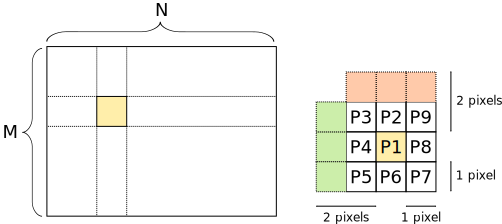
\includegraphics[width=0.9\textwidth]{figs/problem_description}
            \caption{Problem description}
            \label{fig:problem_description}
        \end{figure}

        \subsection{``Hot zone'' detection}
            I am going to use CUDA to accelerate this appliction.
            However, in order find what part to accelerate, I first need to know where the ``hot zones'' of the code are located.
            To study the application, I have written a straightforward single-threaded CPU implementation of the algorithm.

            The code is supplied in Listing~\ref{lst:cpu} for reference.
            To keep the code brief, most input checking code and NULL pointer verifications are not shown here, and I only focus on the main functions of the implementation.
            \newpage

            \lstinputlisting[caption={CPU version}, label={lst:cpu}]{code/cpu_report.cpp}

            \begin{figure}[ht]
                \centering
                \begin{minipage}[t]{.5\textwidth}
                    \centering
                    
\includegraphics[width=0.85\textwidth]{figs/bicycle_binary.png}
                    \caption{$Bicycle: 6409 \times 4139$}
                    \label{fig:bicycle_binary}
                \end{minipage}%
                \begin{minipage}[t]{.5\textwidth}
                    \centering
                    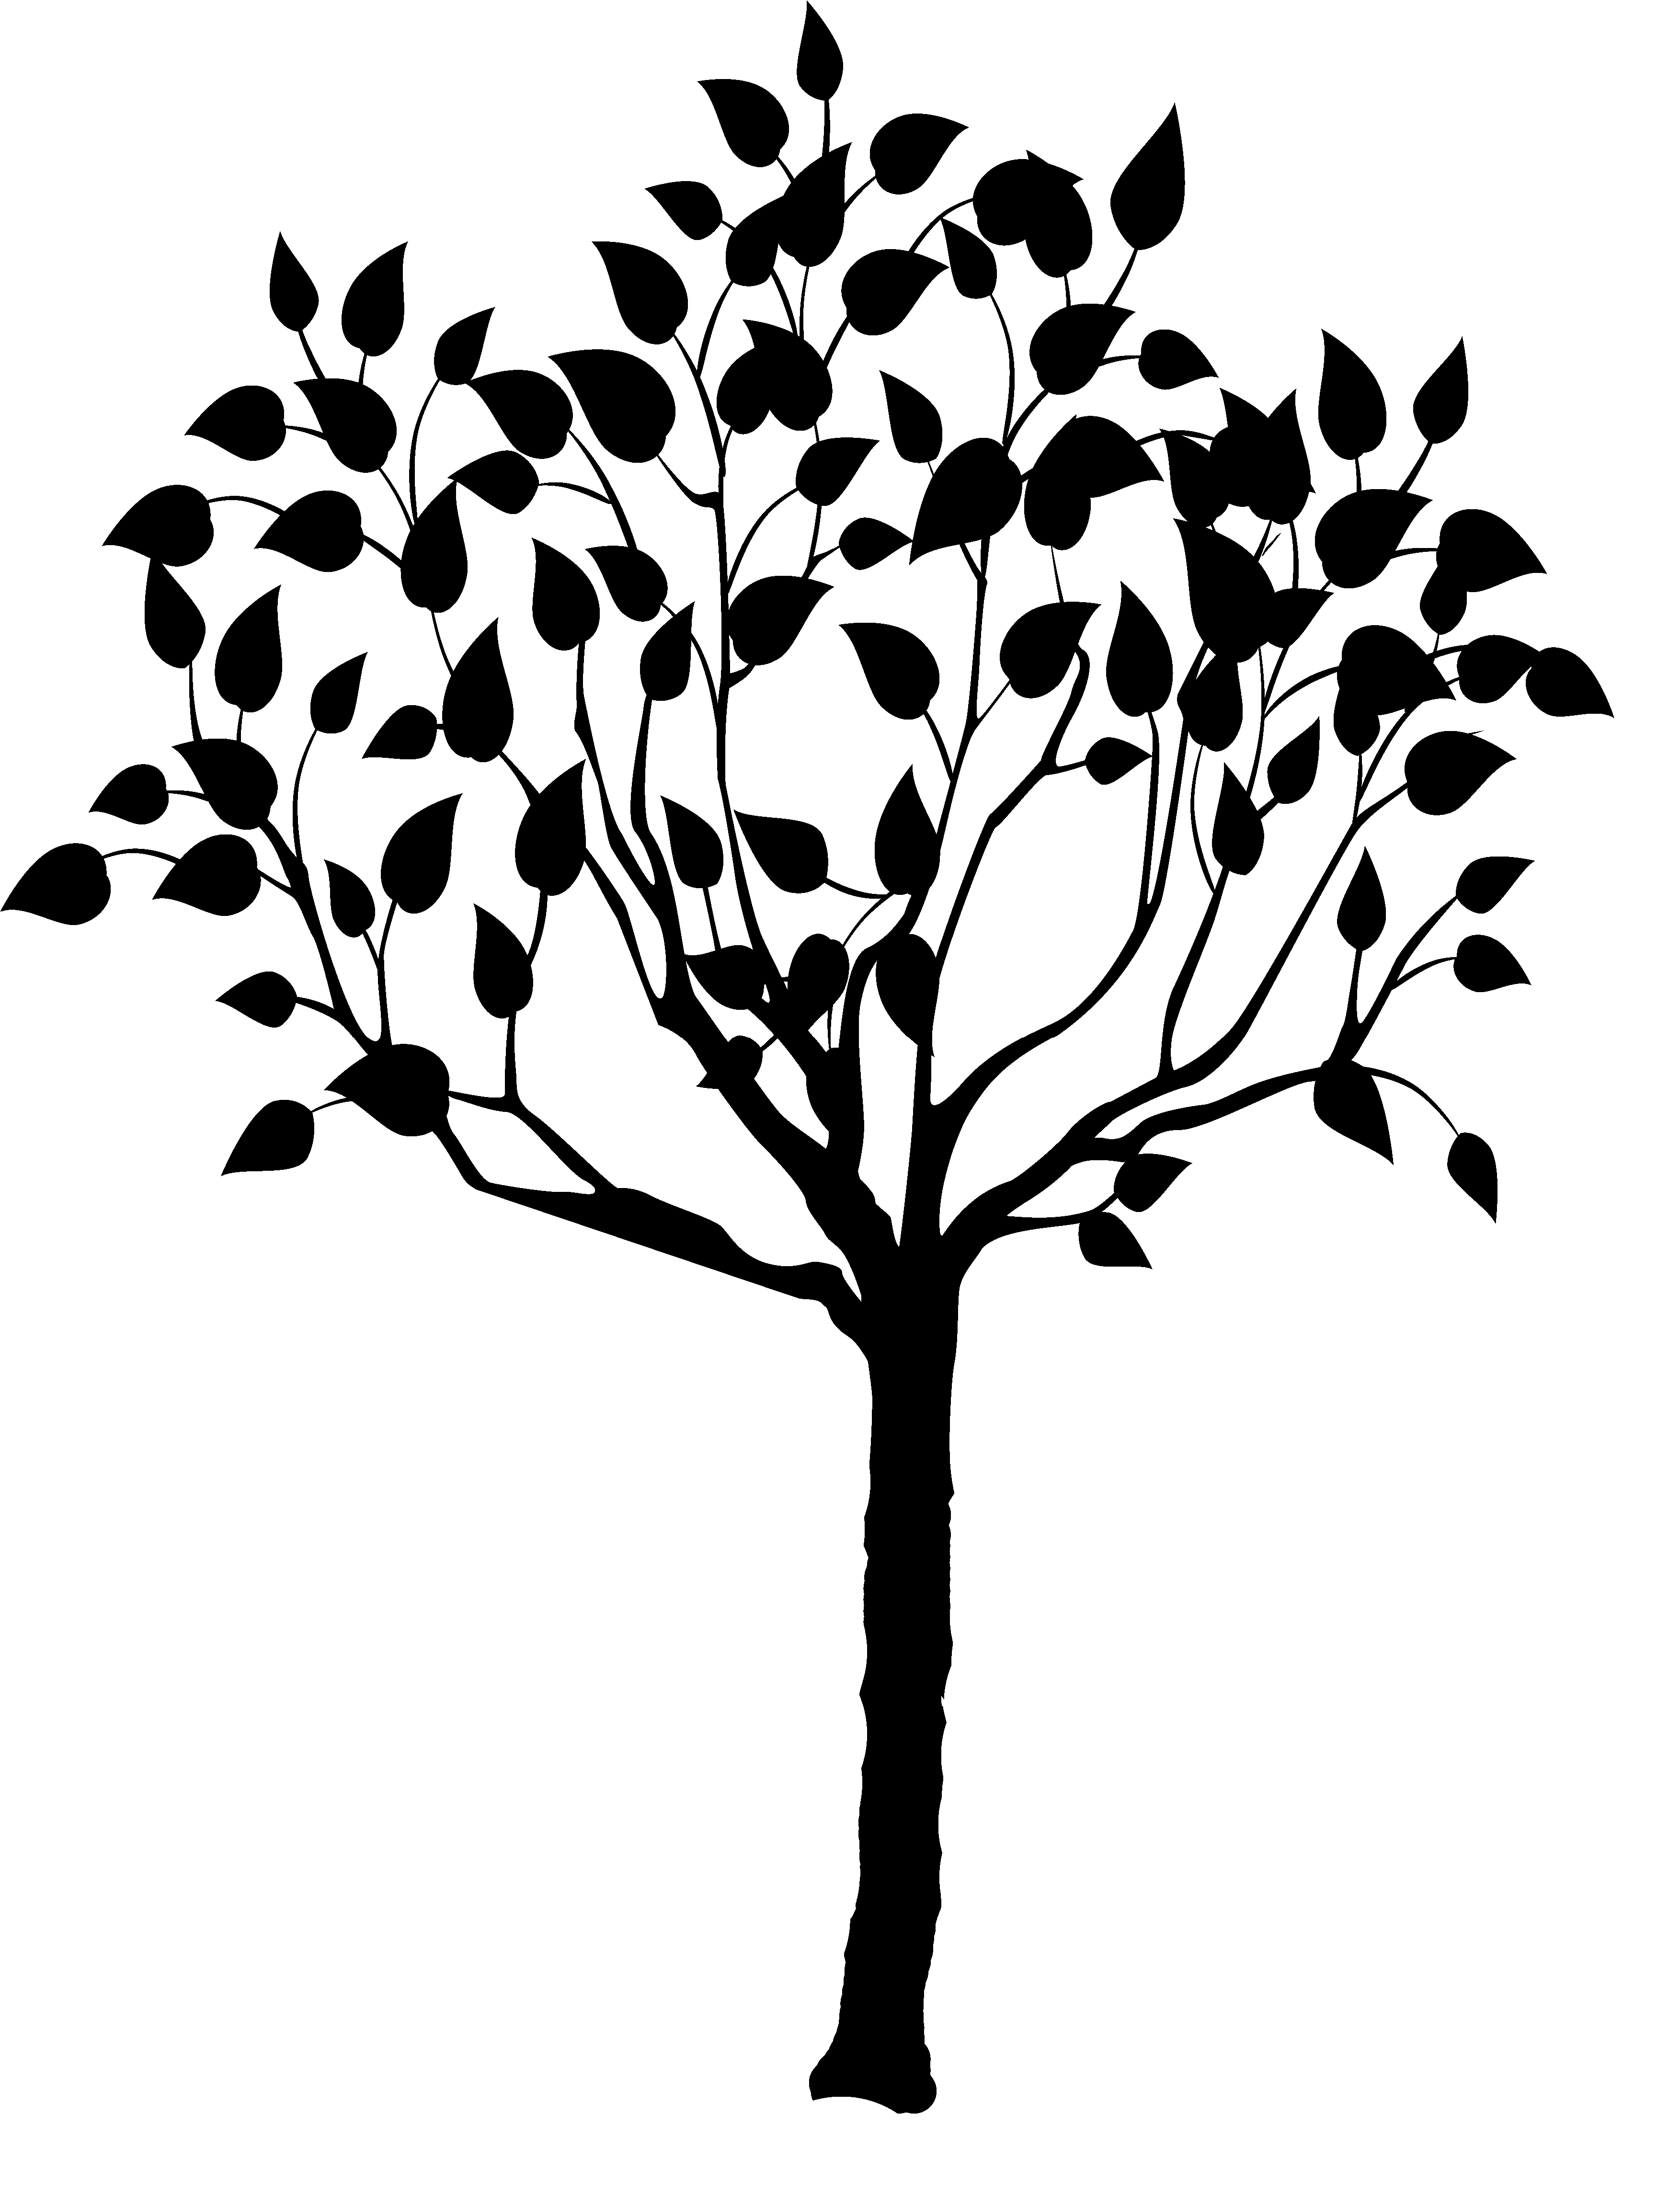
\includegraphics[width=0.6\textwidth]{figs/tree_6_binary.png}
                    \caption{$Tree_{6}: 3507 \times 4582$}
                    \label{fig:tree_6_binary}
                \end{minipage}
            \end{figure}

            \begin{table}[h]
                \centering
                \begin{tabular}{lcccc}
                    \toprule
                                                  & \multicolumn{2}{c}{$Bicycle$} & \multicolumn{2}{c}{$Tree_6$} \\
                    Function                      & Incl. \% & Excl. \%           & Incl. \% & Excl. \%          \\
                    \midrule
                    \verb+main+                   & 100.0    & 0.00               & 100.0    & 0.00              \\
                    \verb+skeletonize+            & 98.62    & 0.00               & 97.91    & 0.00              \\
                    \verb+skeletonize_pass+       & 96.31    & 56.82              & 94.97    & 61.04             \\
                    \verb+wb_transitions_around+  & 39.49    & 39.49              & 33.93    & 33.93             \\
                    \verb+are_identical_bitmaps+  & 2.31     & 2.31               & 2.94     & 2.94              \\
                    \bottomrule
                \end{tabular}
                \caption{CPU profiling data}
                \label{tab:cpu_profiling_data}
            \end{table}

            Table~\ref{tab:cpu_profiling_data} shows some profiling results, as collected by the \emph{Callgrind} profiler when the algorithm is run on the images shown in Figures \ref{fig:bicycle_binary} and \ref{fig:tree_6_binary}.
            Note that optimized code was profiled, so some functions have been automatically inlined by the compiler, and don't show up in the results.

            The two columns show the \emph{inclusive} and \emph{exclusive} time spent in some functions.

            \begin{itemize}
                \item Inclusive time measures the total time spent in a function, \emph{including} time spent executing subfunctions.
                \item Exclusive time measures the total time spent in a function, \emph{excluding} time spent executing subfunctions.
            \end{itemize}

            The results show that more than 97\% of the total CPU execution time is spent in \verb+skeletonize+.
            This function is the ``hot zone'' of the application, and therefore is the function I will try to parallelize.

        \subsection{Complexity analysis}
            To calculate the complexity of the application, I need to know the complexity of all functions.
            Table~\ref{tab:function_complexities} shows the complexity of all functions.

            \begin{table}[h]
            \centering
                \begin{tabular}{lcl}
                    \toprule
                    Function                      & Complexity                    & Explanation                         \\
                    \midrule
                    \verb+black_neighbors_around+ & $\mathcal{O}(1)$              & Straight-line arithmetic            \\
                    \verb+is_outside_image+       & $\mathcal{O}(1)$              & Straight-line arithmetic            \\
                    \verb+P[1-9]_f+               & $\mathcal{O}(1)$              & Straight-line arithmetic            \\
                    \verb+swap_bitmaps+           & $\mathcal{O}(1)$              & Pointer swap                        \\
                    \verb+wb_transitions_around+  & $\mathcal{O}(1)$              & Straight-line arithmetic            \\
                    \verb+are_identical_bitmaps+  & $\mathcal{O}(M \cdot N)$      & Iterates over all pixels            \\
                    \verb+skeletonize_pass+       & $\mathcal{O}(M \cdot N)$      & Iterates over all pixels            \\
                    \verb+skeletonize+            & $\geq \mathcal{O}(M \cdot N)$ & Iterates until image stops changing \\
                    \bottomrule
                \end{tabular}
                \caption{Function complexities}
                \label{tab:function_complexities}
            \end{table}

            The main issue for determining the application's complexity lies in the fact that \verb+skeletonize+'s ending condition depends on the input image.
            The algorithm is data-dependant, and it isn't possible to give an accurate estimate of the complexity.

            However, I have experimentally observed that the number of iterations is proportional to $$\frac{1}{2} \times \max(w_{b}, h_{b}),$$ where $w_{b}$ and $h_{b}$ represent the width and height of the ``thickest'' black zone in the image, respectively.

            Therefore, the overall algorithms's complexity is $\mathcal{O}(M \cdot N \cdot \max(w_{b}, h_{b}))$.

        \subsection{Theoretical maximum speedup}
            \label{sec:theoretical_maximum_speedup}
            Amdahl's law says that if $P$ is the proportion of a program that can be made parallel, and $(1-P)$ is the proportion that cannot be parallelized, then the maximum speedup that can be obtained by using $N$ processors is

            $$ S(N) = \frac{1}{(1-P) + \frac{P}{N}} $$

            The part of my application that I want to parallelize is \verb+skeletonize+, which takes roughly 97\% of the total execution time.
            By substituting this value in the equation, I get

            $$ S(N) = \frac{1}{(1-0.97) + \frac{0.97}{N}} $$

            To find the theoretical maximum speedup, I can assume that the problem is ``infinitely'' parallelizable by setting $N$ to $\infty$.

            $$ S(N) = \frac{1}{(1-0.97)} = 33.33 $$

            Therefore, the theoretical maximum speedup that can be achieved is around 33.33.

        \subsection{Reference machine}
            The actual speedup obtained depends on the reference machine measurements will be performed on.
            I was granted access to one of LACALs servers for this project.
            Its specifications are listed in Table~\ref{tab:reference_machine_specifications}.

            \begin{table}[h]
            \centering
                \begin{tabular}{lccc}
                    \toprule
                    Device & Specifications         & Cores    & Speed   \\
                    \midrule
                    CPU    & Intel Core i7-2600K    & 4        & 3.4 GHz \\
                    GPU    & Nvidia GeForce GTX 580 & 512      & 772 MHz \\
                    Bus    & PCIe 2.0 $\times$ 16   & \verb+-+ & 8 GB/s  \\
                    \bottomrule
                \end{tabular}
                \caption{Reference machine specifications}
                    \label{tab:reference_machine_specifications}
            \end{table}

            All CPU \& GPU implementations were compiled with \verb|-O3| to take advantage of any compile-time optimizations.
            The project was built with the tools contained in CUDA SDK v5.0.

    \section{Parallelization solutions}
        As stated earlier, I will parallelize the \verb+skeletonize+ function, which calculates a new image by iterating over all its pixels and applying a thinning operation.
        The only parallelizable parts of this function are \verb+skeletonize_pass+, and \verb+are_identical_bitmaps+, as all the other ones are straight-line arithmetic, and are $\mathcal{O}(1)$.

        In order to map the problem to the GPU, I decided to assign each pixel of the image to one thread which will be responsible for computing the next value of that single pixel.

        Note that the \verb+while+ loop of the calling \verb+skeletonize+ function cannot be part of a CUDA kernel.
        The reason is that the image is going to be split into multiple blocks for the computation, and that CUDA does not currently support synchronizing threads across multiple blocks.

        If we suppose the \verb+while+ loop was inside the CUDA kernel, then it is possible for threads of one block to already be on their \emph{second} pixel computation, whereas other blocks haven't finished their \emph{first} pixel computation.
        At the moment, there are only two ways to synchronize threads across multiple blocks:

        \begin{enumerate}
            \item Atomically use a variable in device global memory to check if every thread has finished one pass of their thinning opreation. This is very slow, as many threads will be accessing the same global memory location.
            \item Terminate the kernel and launch it again. This is easier to do and is faster. The CUDA runtime guarantees that all blocks have terminated upon kernel termination. Additionally, multiple posts on Nvidia forums claim that a kernel invocation is lightweight for the host. I will use this method.
        \end{enumerate}

        Note that all CUDA binaries produced in this project take 2 arguments as input:

        \begin{enumerate}
            \item Horizonatal block dimension
            \item Vertical block dimension
        \end{enumerate}

        The grid dimensions are computed from the provided block dimensions above in order to cover the entire image.

        CUDA devices have multiple different memories, each with different characteristics.
        To obtain a good speedup, one must select the appropriate memory for their application.
        I will present 4 parallel solutions, each \emph{generally} faster than the previous by leveraging the different CUDA memories.

        \subsection{GPU 1}
            \label{sec:solution_1}

            \subsubsection{Idea}
                This first parallel implementation consists of simply transforming \verb+skeletonize_pass+ into a CUDA kernel.
                This is straight-forward and can be implemented by only using the CUDA device's global memory.

                % Listing~\ref{lst:gpu1} shows a subset of this implementation.
                % \lstinputlisting[caption={GPU version 1}, label={lst:gpu1}]{code/gpu1_report.cu}

            \subsubsection{Analysis}
                This implementation suffers from a high amount of transfer time between the host and the device.
                Indeed, at every iteration, both the \verb+src+ and \verb+dst+ bitmaps are transferred back to the host.

                Figure~\ref{fig:black_gpu1_timing_diagram} shows the timing diagram of $GPU_{1}$ during 1 iteration of the \verb+while+ loop in the \verb+skeletonize+ function (taken from the Nvidia Visual Profiler) when the application was run on a $8000~\times~8000$ \emph{full} black image.
                Table~\ref{tab:black_gpu1_timing_diagram} summarizes the results.

                A 100 \% black image was chosen in order to have high amount of arithmetic done in both the CPU and GPU versions.

                \begin{figure}[ht]
                    \centering
                    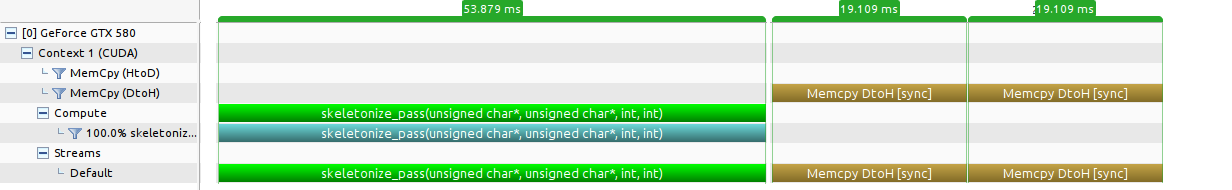
\includegraphics[width=\textwidth]{figs/black_gpu1_timing_diagram.png}
                    \caption{$GPU_{1}$ timing diagram during 1 iteration ($8000 \times 8000$ full black image).}
                    \label{fig:black_gpu1_timing_diagram}
                \end{figure}

                The gaps between the different events shown on the timing diagram are due to the CUDA API overhead.

                \begin{table}[ht]
                    \centering
                    \begin{tabular}{lcc}
                        \toprule
                        Function                      & Time spent (\%) & Time spent (ms) \\
                        \midrule
                        \verb+skeletonize_pass+       & 57.95           & 53.879          \\
                        \verb+cudaMemcpyDeviceToHost+ & 41.10           & 38.218          \\
                        \midrule
                        \verb+Total+                  & 99.04           & 92.983          \\
                        \bottomrule
                    \end{tabular}
                    \caption{$GPU_{1}$ profiling data during 1 iteration ($8000 \times 8000$ full black image).}
                    \label{tab:black_gpu1_timing_diagram}
                \end{table}

                % \begin{figure}[ht]
                %     \centering
                %     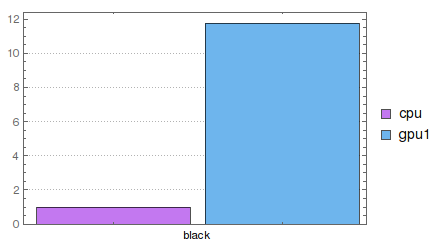
\includegraphics[width=0.5\textwidth]{figs/black_cpu_gpu1_speedup.png}
                %     \caption{Total speedup ($8000 \times 8000$ full black image, 4001 iterations).}
                %     \label{fig:black_cpu_gpu1_speedup}
                % \end{figure}

                As one can see, around 41 \% of the total time spent in each iteration is used to transfer data to the host.
                This issue brings me to my next implementation.

        \subsection{GPU 2}
            \label{sec:solution_2}

            \subsubsection{Idea}
                This second solution is identical to the one presented in \ref{sec:solution_1}, but it addresses the huge transfer time issue between the host and the device.

                The reason data was being sent back to the host was for it to decide whether the 2 images have changed during the iteration.
                We can avoid sending the data to the host by making the GPU compute the images' equality.

                This can be accomplished by performing a \emph{reduction} algorithm on the GPU to compute a single flag from the content of both images.
                This flag would indicate whether the images have changed during the iteration.
                All that would need to be done at the end of an iteration would be to transfer this flag back to the host, in order for it to decide whether to relaunch the \verb+skeletonize_pass+ kernel.

                % Listing~\ref{lst:gpu2} shows a subset of this implementation.

                The \verb+skeletonize_pass+ kernel remains unchanged, and only code for performing the reduction is added.
                To do this, 2 new kernels are added:
                \begin{itemize}
                    \item \verb+pixel_equality+, which tests the equality of each element in the \verb+src+ and \verb+dst+ bitmaps, and stores this information in another array of the same size as the images, \verb+equ+. Concretely, it calculates \verb+equ[i] = (src[i] == dst[i])+.
                    \item \verb+and_reduction+, which reads the \verb+equ+ array and performs a binary AND reduction over it.
                \end{itemize}

                Note that the reduction code uses a small chunk of shared memory to perform the algorithm before writing the result back to global memory.
                Also, depending on the size of the image, the reduction may not be finished in 1 iteration, so multiple successive reductions are necessary to obtain the final flag.
                This could be an issue, as the CUDA API overhead can add up, however, each reduction reduces the size of the output by \verb+(blockDim.x * blockDim.y)+, so few passes are necessary (for example, with a $16 \times 16$ block size, the image gets reduced 256 times each iteration).

                % \lstinputlisting[caption={GPU version 2}, label={lst:gpu2}]{code/gpu2_report.cu}

            \subsubsection{Analysis}
                Figure~\ref{fig:black_gpu2_timing_diagram} shows the timing diagram of $GPU_{2}$ during 1 iteration of the \verb+while+ loop.
                Table~\ref{tab:black_gpu2_timing_diagram} summarizes the results.

                \begin{figure}[h]
                    \centering
                    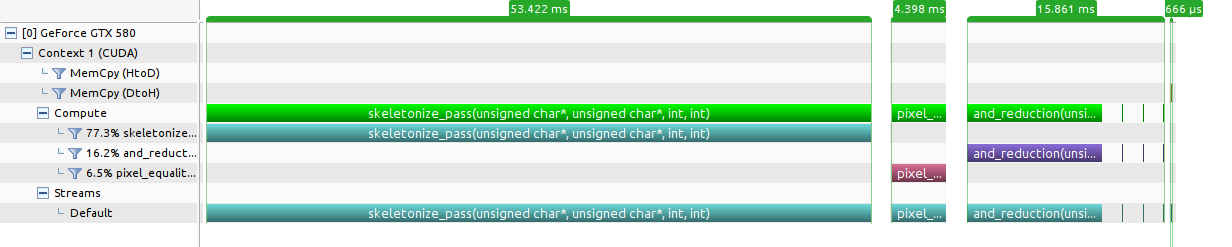
\includegraphics[width=\textwidth]{figs/black_gpu2_timing_diagram.png}
                    \caption{$GPU_{2}$ timing diagram during 1 iteration ($8000 \times 8000$ full black image).}
                    \label{fig:black_gpu2_timing_diagram}
                \end{figure}

                \begin{table}[ht]
                    \centering
                    \begin{tabular}{lcc}
                        \toprule
                        Function                      & Time spent (\%) & Time spent (ms) \\
                        \midrule
                        \verb+skeletonize_pass+       & 68.77           & 53.422          \\
                        \verb+pixel_equality+         & 5.66            & 4.398           \\
                        \verb+and_reduction+          & 20.42           & 15.861          \\
                        \verb+cudaMemcpyDeviceToHost+ & 0.21            & 0.161           \\
                        \midrule
                        \verb+Total+                  & 95.06           & 77.682          \\
                        \bottomrule
                    \end{tabular}
                    \caption{$GPU_{2}$ profiling data during 1 iteration ($8000 \times 8000$ full black image).}
                    \label{tab:black_gpu2_timing_diagram}
                \end{table}

                % \begin{figure}[ht]
                %     \centering
                %     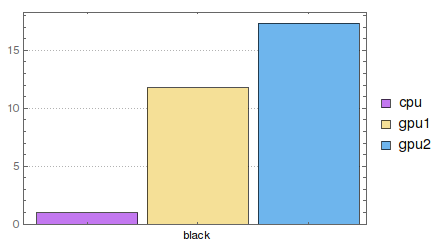
\includegraphics[width=0.5\textwidth]{figs/black_cpu_gpu1_gpu2_speedup.png}
                %     \caption{Total speedup ($8000 \times 8000$ full black image, 4001 iterations).}
                %     \label{fig:black_cpu_gpu1_gpu2_speedup}
                % \end{figure}

                This version solves the memory copy issue, as transfers between then host and the device only account for 0.2 \% of the total time spent during an iteration.

                However, this version still suffers from one issue: global memory contention.
                Each pixel in \verb+dst+ requires the values of 15 pixels in \verb+src+ in order to be computed.
                Therefore, each thread in a block is going to somehow load these 15 values from global memory.
                Additionally, these pixel valus are not merely read a single time, but are accessed very often.
                Indeed, neighboring threads will also load most of the same values, resulting in even more global memory accesses.
                This CUDA kernel is very likely to suffer from latency issues due to contention in global memory.

        \subsection{GPU 3}
            \label{sec:solution_3}

            \subsubsection{Idea}
                The idea here is to load the pixels that lie in a block's tile to its \emph{shared} memory.
                All threads in the block will heavily use the contents of the shared memory to perform their computation.

                The reduction kernel already loads data into shared memory, so the issue is in \verb+skeletonize_pass+.
                In the \verb+and_reduction+ kernel, every unique data element is read once.
                As such, reductions don't have high arithmetic intensity.

                However, each thread in \verb+skeletonize_pass+ reads the value of 15 neighboring pixels multiple times.
                There is a good opportunity to avoid many global memory reads by using shared memory.
                In this version, the host allocates \verb|(blockDim.x + 3) * (blockDim.y + 3)| bytes of shared memory for each tile in \verb+skeletonize_pass+.
                The \verb|+3| is due to the surrounding pixel values that are also needed for this tile.
                Each thread in the ``center'' of the tile is responsible for loading 1 pixel value into shared memory, but the threads on the boundaries load 3, 4, 6, or 9 pixels depending on their position (corner, border, \ldots).

            \subsubsection{Analysis}
                Figure~\ref{fig:black_gpu3_timing_diagram} shows the timing diagram of $GPU_{3}$ during 1 iteration of the \verb+while+ loop.
                Table~\ref{tab:black_gpu3_timing_diagram} summarizes the results.

                \begin{figure}[h]
                    \centering
                    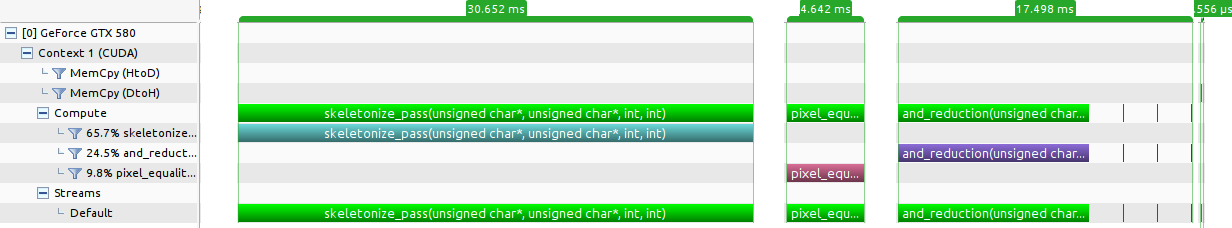
\includegraphics[width=\textwidth]{figs/black_gpu3_timing_diagram.png}
                    \caption{$GPU_{3}$ timing diagram during 1 iteration ($8000 \times 8000$ full black image).}
                    \label{fig:black_gpu3_timing_diagram}
                \end{figure}

                \begin{table}[ht]
                    \centering
                    \begin{tabular}{lcc}
                        \toprule
                        Function                      & Time spent (\%) & Time spent (ms) \\
                        \midrule
                        \verb+skeletonize_pass+       & 53.37           & 30.652          \\
                        \verb+pixel_equality+         & 8.08            & 4.642           \\
                        \verb+and_reduction+          & 30.47           & 17.498          \\
                        \verb+cudaMemcpyDeviceToHost+ & 0.31            & 0.179           \\
                        \midrule
                        \verb+Total+                  & 92.23           & 57.435          \\
                        \bottomrule
                    \end{tabular}
                    \caption{$GPU_{3}$ profiling data during 1 iteration ($8000 \times 8000$ full black image).}
                    \label{tab:black_gpu3_timing_diagram}
                \end{table}

                Compared to $GPU_{2}$, this version reduces the time spent in \verb+skeletonize_pass+ from 53.422 ms to 30.652 ms, which is a 42.6 \% improvement.
                It is not as I expected though. I was expecting a reduction of around 93 \% (15 \emph{times} less loads from global memory), but it seems that the arithmetic is not enough to hide so much global memory latency.
                In future work, one should give more work to each thread to hide more of the global memory access latency.

                There is not much more that can be done in this version to speed up \verb+skeletonize_pass+. However, by looking at the time spent in \% in Table~\ref{tab:black_gpu3_timing_diagram}, we can see that \verb+and_reduction+ is starting to take a more important percentage of the total execution time (30.47~\% vs 20.42~\% in $GPU_{2}$).

                This brings me to my final implementation.

        \subsection{GPU 4}
            \label{sec:solution_4}

            \subsubsection{Idea}
                The state of the code until now is that \verb+skeletonize_pass+ calculates the future value of each pixel, \verb+pixel_equality+ computes an array \verb+equ[i] = (src[i] == dst[i])+, and \verb+and_reduction+ reduces \verb+equ+ to a single value.

                The issue is that \verb+pixel_equality+ and \verb+and_reduction+ are kernels, so they are forced to load data from global memory, and cannot use any shared memory loaded by \verb+skeletonize_pass+.

                However, \verb+skeletonize_pass+ has everything the first iteration of \verb+and_reduction+ needs, namely

                \begin{itemize}
                    \item \verb+src+ in shared memory
                    \item Future value of \verb+dst+ in a register
                \end{itemize}

                If we could somehow do the first iteration of the reduction with these shared memory values, we could avoid having to compute the \verb+pixel_equality+ kernel completely, and would get rid of the big first chunk of \verb+and_reduction+, which is the biggest part.
                The subsequent iterations of \verb+and_reduction+ are small, and are only affected by the CUDA API overhead.

                In order to do this, the host must allocate more shared memory on the device.
                Now, it allocates \verb|(((blockDim.x + 3) * (blockDim.y + 3)) + (blockDim.x * blockDim.y))| bytes of shared memory, which is enough to hold the values of \verb+src+, and of \verb+equ+ for this tile.

                At the end of \verb+skeletonize_pass+, \verb+equ+ is set from the values of \verb+src+ and \verb+dst+ stored in shared memory.
                Then, I perform the first iteration of the reduction on the \emph{shared} value of \verb+equ+.
                This operation lengthens \verb+skeletonize_pass+ compared to $GPU_{3}$, but it avoids more global memory loads.

                However, we are not done yet. We are only using \verb+equ+ at the end of \verb+skeletonize_pass+, but we could also use it at the beginning to mimic an optimization done on the CPU algorithm.
                The CPU's greatest optimization is that it has the ability to skip any pixels that are white, so it can rapidly get to the areas of the image where work is to be done.
                On the GPU, after \verb+src+ is loaded into shared memory, we can use \verb+equ+ to check if the tile only contains white pixels. If it is the case, then nothing needs to be done, and we can skip the skeletonization part of the tile entirely.

                This optimization is also included in $GPU_{4}$, and has the advantage that the number of global memory stores decreases after each iteration, making each one slightly faster than the previous (more on this in section~\ref{sec:detailed_analysis}).

            \subsubsection{Analysis}
                Figure~\ref{fig:black_gpu4_timing_diagram} shows the timing diagram of $GPU_{4}$ during 1 iteration of the \verb+while+ loop.
                Table~\ref{tab:black_gpu4_timing_diagram} summarizes the results.

                \begin{figure}[h]
                    \centering
                    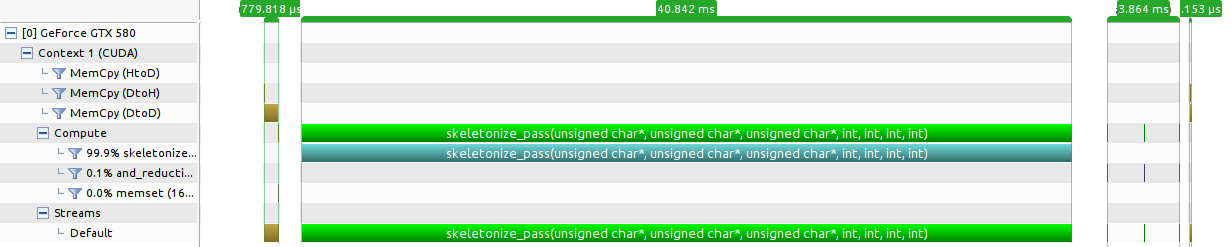
\includegraphics[width=\textwidth]{figs/black_gpu4_timing_diagram.png}
                    \caption{$GPU_{4}$ timing diagram during 1 iteration ($8000 \times 8000$ full black image).}
                    \label{fig:black_gpu4_timing_diagram}
                \end{figure}

                \begin{table}[ht]
                    \centering
                    \begin{tabular}{lcc}
                        \toprule
                        Function                        & Time spent (\%) & Time spent (ms) \\
                        \midrule
                        \verb+cudaMemcpyDeviceToDevice+ & 1.58            & 0.780           \\
                        \verb+cudaMemset+               & 0.22            & 0.106           \\
                        \verb+skeletonize_pass+         & 82.92           & 40.842          \\
                        \verb+and_reduction+            & 7.84            & 3.864           \\
                        \verb+cudaMemcpyDeviceToHost+   & 0.22            & 0.106           \\
                        \midrule
                        \verb+Total+                    & 92.78           & 49.255          \\
                        \bottomrule
                    \end{tabular}
                    \caption{$GPU_{4}$ profiling data during 1 iteration ($8000 \times 8000$ full black image).}
                    \label{tab:black_gpu4_timing_diagram}
                \end{table}

                As we can see, the total time spent in \verb+and_reduction+ is greatly reduced, and the overall execution time of an iteration has decreased by roughly 14.24~\% (depends on the image).

    \section{Detailed Analysis}
        \label{sec:detailed_analysis}
        I will give an analysis for the solution given in \ref{sec:solution_4}.

        \begin{figure}[ht]
            \begin{subfigure}[t]{0.5\linewidth}
                \centering
                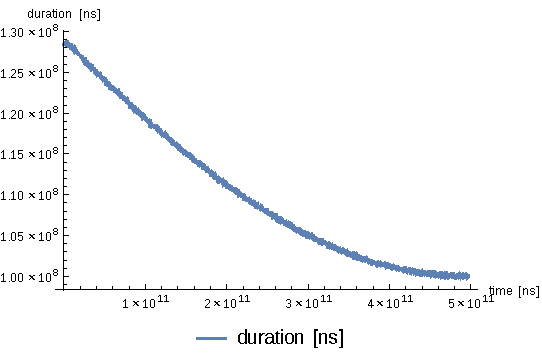
\includegraphics[width=\linewidth]{figs/black_iteration_duration_plot.pdf}
                \caption{Duration of 1 iteration over time.}
                \label{fig:black_duration_of_1_iteration_over_time}
                \vspace{4ex}
            \end{subfigure}%%
            \begin{subfigure}[t]{0.5\linewidth}
                \centering
                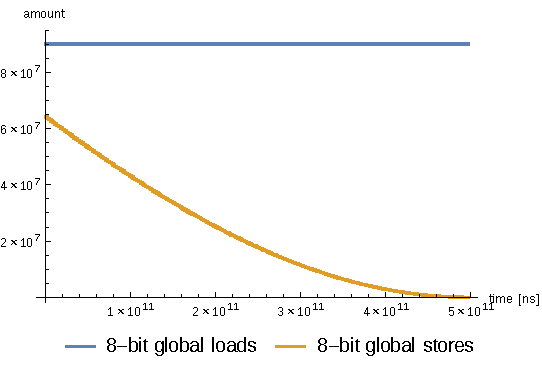
\includegraphics[width=\linewidth]{figs/black_iteration_global_load_store_plot.pdf}
                \caption{Number of global loads/stores over time.}
                \label{fig:black_number_of_global_loads_stores_over_time}
            \end{subfigure}
            \begin{subfigure}[t]{0.5\linewidth}
                \centering
                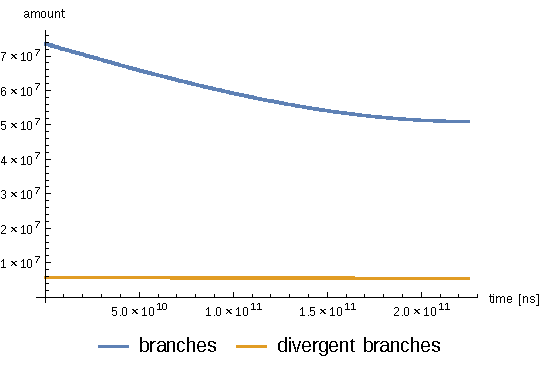
\includegraphics[width=\linewidth]{figs/black_iteration_branch_and_divergent_branch_plot.pdf}
                \caption{Number of normal/divergent branches over time.}
                \label{fig:black_number_of_branches_over_time}
            \end{subfigure}%%
            \begin{subfigure}[t]{0.5\linewidth}
                \centering
                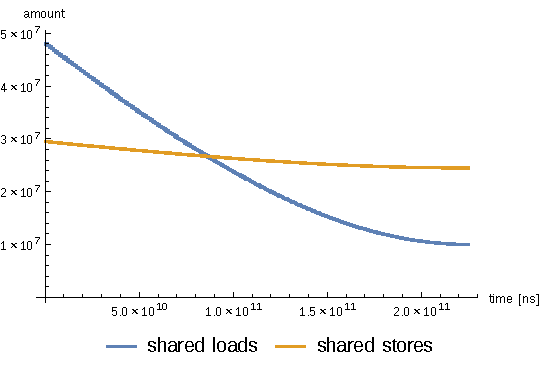
\includegraphics[width=\linewidth]{figs/black_iteration_shared_load_store_plot.pdf}
                \caption{Number of shared loads/stores over time.}
                \label{fig:black_number_of_shared_loads_stores_over_time}
                \vspace{4ex}
            \end{subfigure}
            \caption{Evolution of each iteration of skeletonize\_pass kernel over time.}
            \label{fig:evolution_of_each_iteration_of_skeletonize_pass_kernel_over_time}
        \end{figure}

        Figure~\ref{fig:black_duration_of_1_iteration_over_time} shows that the duration of each iteration of \verb+skeletonize_pass+ reduces by around 30~\% due to the reduced global memory operations.

        Figure~\ref{fig:black_number_of_global_loads_stores_over_time} shows that the number of global stores decreases until 0.
        However, the number of global loads stays constant, as the image must be read at each iteration.

        Figure~\ref{fig:black_number_of_shared_loads_stores_over_time} shows that once the shared memory is loaded, its use decreases over time as the image becomes more and more white.
        This is normal, as the skeletonization algorithm is not run on a white block of pixels.

        Figure~\ref{fig:gpu4_execution_time_with_various_block_sizes} shows how the execution time varies when different block sizes are used.
        Due to how I implemented the algorithm, it isn't possible to specify grid sizes, so it isn't possible to artificially limit the number of cores used in the application.
        The only thing that can be done is vary the number of threads that are contained in a block.
        We can see that the sweet spot for the execution time is when 128 threads are used per block.

        Finally, Figure~\ref{fig:speedup_benchmarks_with_various_images} summarizes the speedups obtained across all implementations over a wide range of images.
        It is interesting to see that the speedup is indeed correlated with the width and height of the ``thickest'' black zone of the image. The images are available in the CD that came with the report.

        \begin{figure}[h]
            \centering
            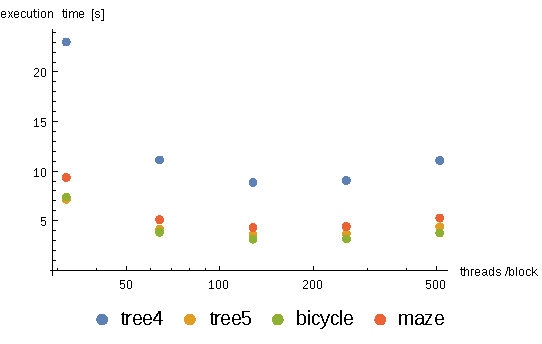
\includegraphics[width=0.75\textwidth]{figs/block_size_plot.pdf}
            \caption{$GPU_{4}$ execution time with various block sizes.}
            \label{fig:gpu4_execution_time_with_various_block_sizes}
        \end{figure}

        \begin{figure}[h]
            \centering
            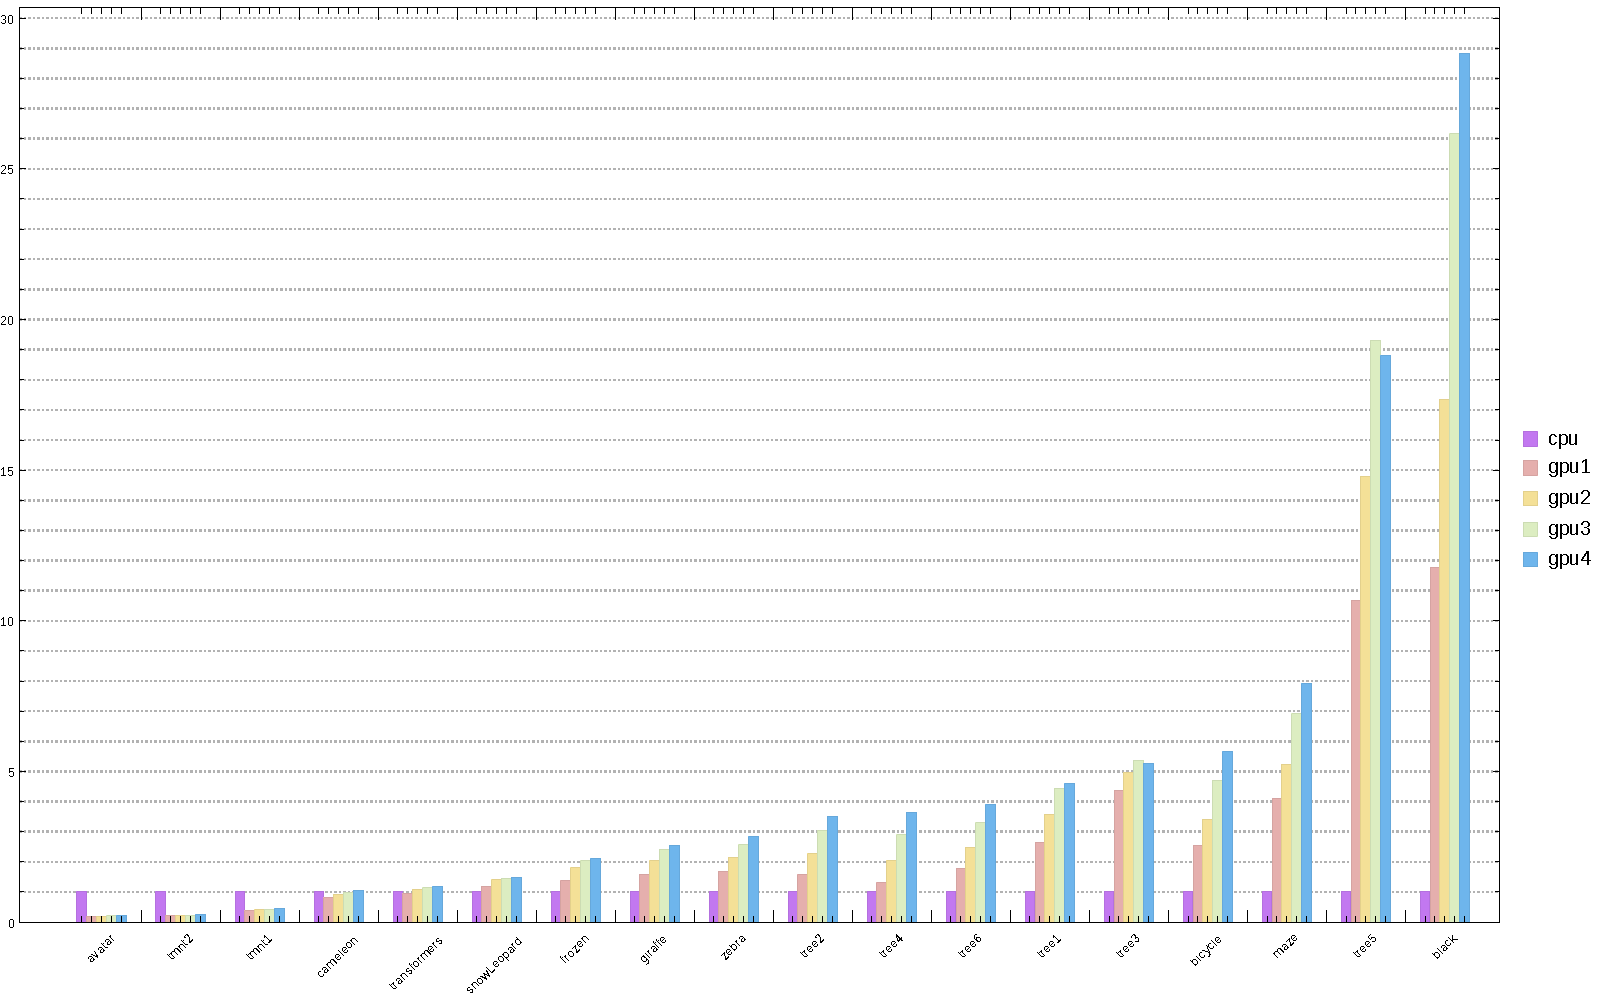
\includegraphics[width=\textwidth]{figs/benchmarks_barplot.pdf}
            \caption{Speedup benchmarks with various images, from slowest to fastest.}
            \label{fig:speedup_benchmarks_with_various_images}
        \end{figure}

        The closest we get to the maximum theoretical speedup is around 29 times, which is close to the 33.3 times we predicted, but only when an image has many black pixels to give an equivalent ``sense'' of work to both the CPU and the GPU implementations.

        We can put this in contrast by also analyzing the speedup obtained if the serial algorithm didn't skip any white pixels. If I profile the serial code with such an algorithm, I see that more than 99.2~\% of the total execution time is spent in \verb+skeletonize+, which can theoretically give a maximum speedup of 125.

        Figure~\ref{fig:speedup_benchmarks_with_various_images_unoptimized} shows some results with an unoptimized serial algorithm, and we can clearly see that the speedup is much closer to the theoretical result, as the problem almost scales perfectly with the size of the image.

        \begin{figure}[h]
            \centering
            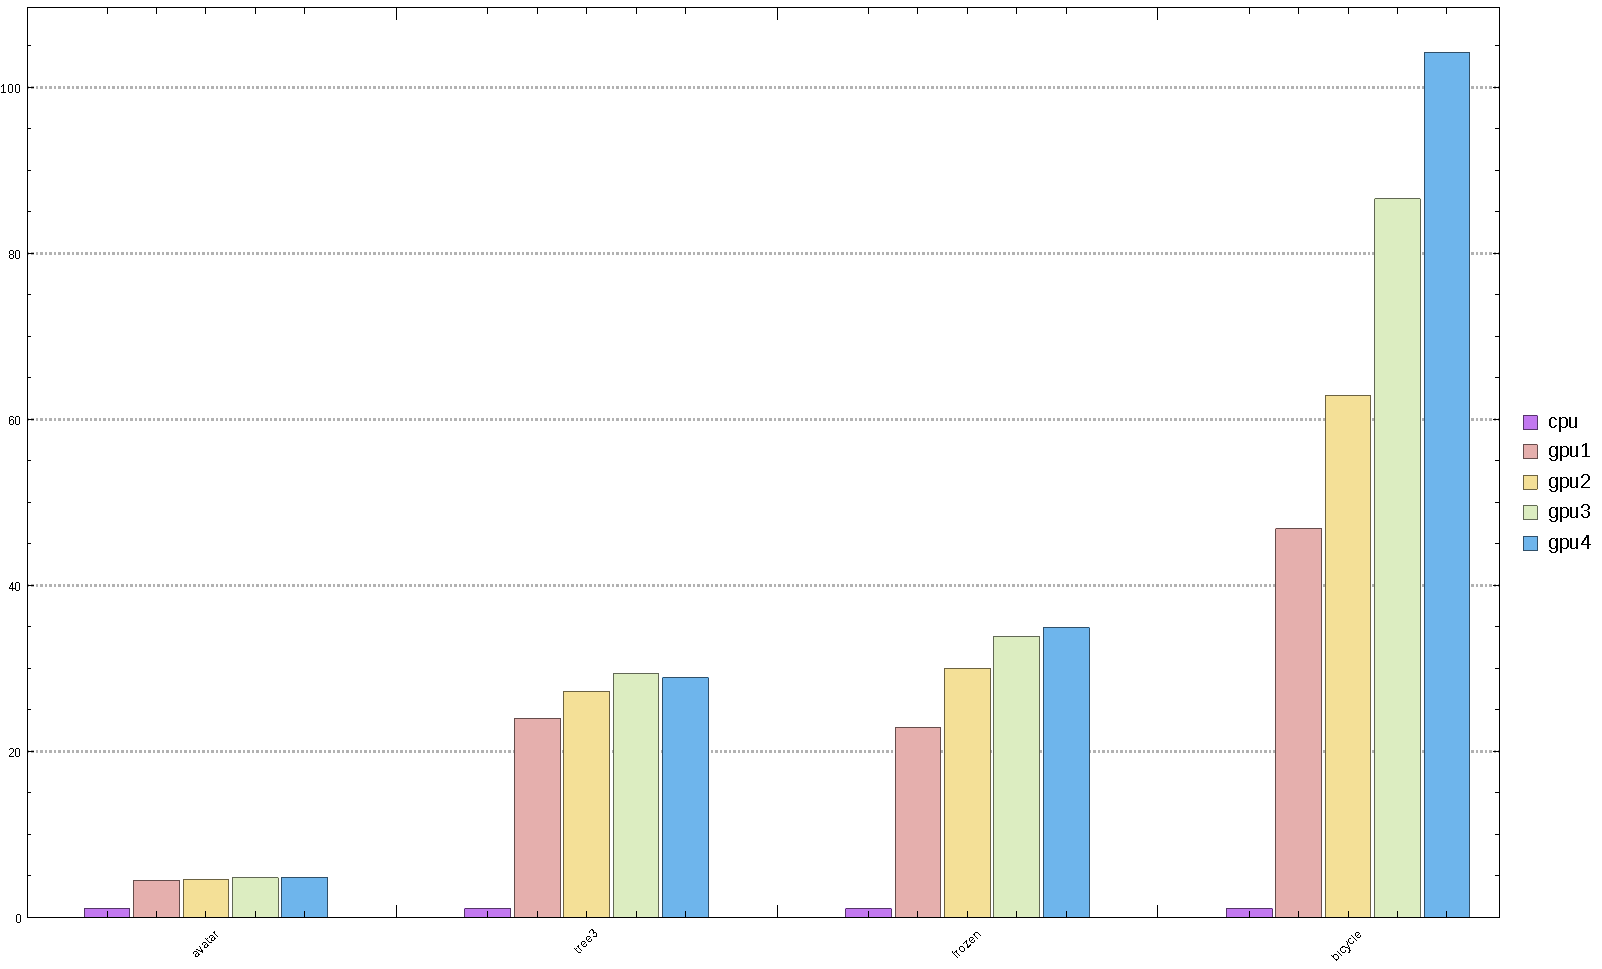
\includegraphics[width=\textwidth]{figs/benchmarks_barplot_unoptimized.pdf}
            \caption{Speedup benchmarks with various images, from slowest to fastest (no skipping white pixels in serial code).}
            \label{fig:speedup_benchmarks_with_various_images_unoptimized}
        \end{figure}

        \section{Conclusion}
            In section~\ref{sec:theoretical_maximum_speedup}, we calculated that the maximum speedup possible is 33.3.
            This computation was based upon a skeletonization algorithm where each pixel is \emph{treated} irrespective of its color.
            However, in practice, some optimizations can be done to speed up the computation, the most prominent of which is skipping any white pixels in the serial version of the code.
            This optimization can distort the real speedup obtained, and it was easily visible in the benchmarks of Figure~\ref{fig:speedup_benchmarks_with_various_images}.
            As we saw in Figure~\ref{fig:speedup_benchmarks_with_various_images_unoptimized}, the theoretical speedups are much easier to achieve when the serial code and the parallel code truly follow the exact same algorithm.

            However, algorithms are made to be fast, so it is cheating to compare a parallel implementation against an intentionally slow serial one.
            Indeed, parallel implementations have to be tested against their fastest serial equivalent to measure true speedups.

\end{document}
